Analizando los resultados obtenidos en el punto anterior, nos dimos cuenta que esa clave presentaba muchos inconvenientes y
decidimos utilizar otro índice simple, en este caso la fecha, que resultó más interesante. A medida que se insertaron los 
datos se puede observar como se produce el balanceo de shards a través de la división y migración de los chunks, ya que es una clave con 
cardinalidad alta. Hay que tener en cuenta que los datos fueron generados de forma aleatoria, quizás en un caso real las fechas serían 
consecutivas lo que deriva en que las inserciones apunten al mismo shard.

\begin{figure}[h!]
 \centering
 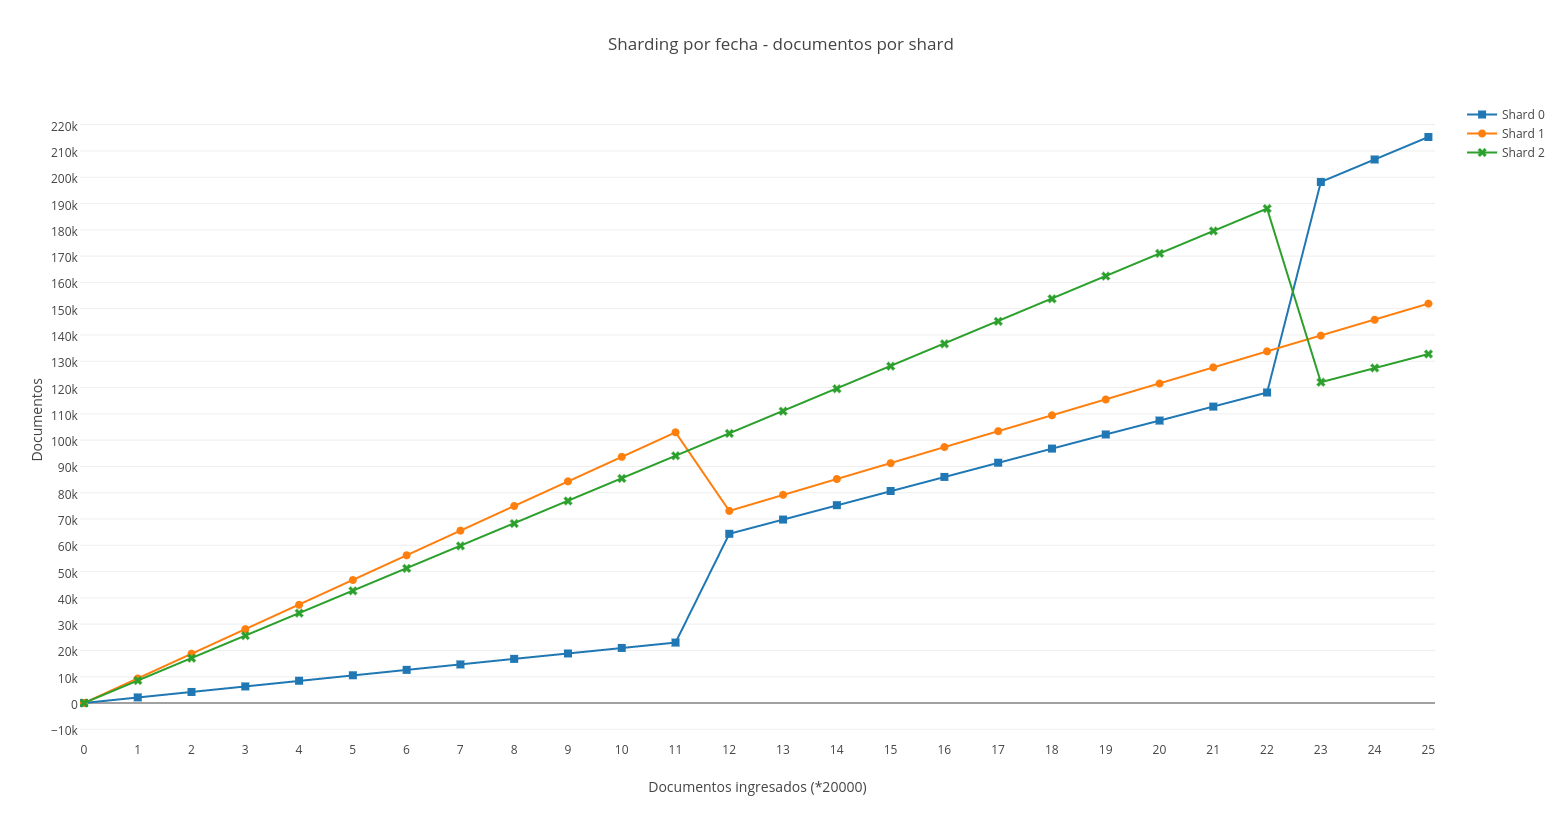
\includegraphics[scale=0.3,keepaspectratio=true]{./fecha-documentos-por-shard.png}
 \caption{Documentos por shard}
\end{figure}

Aquí se observa como se distribuye la carga de datos por shard, no es una distribución perfectamente uniforme pero crecen en general al mismo ritmo. Los cambios bruscos
se deben a migraciones de datos, posiblemente por un chunk muy grande que fue dividido y luego una parte migrada a otro shard.

\begin{figure}[h!]
 \centering
 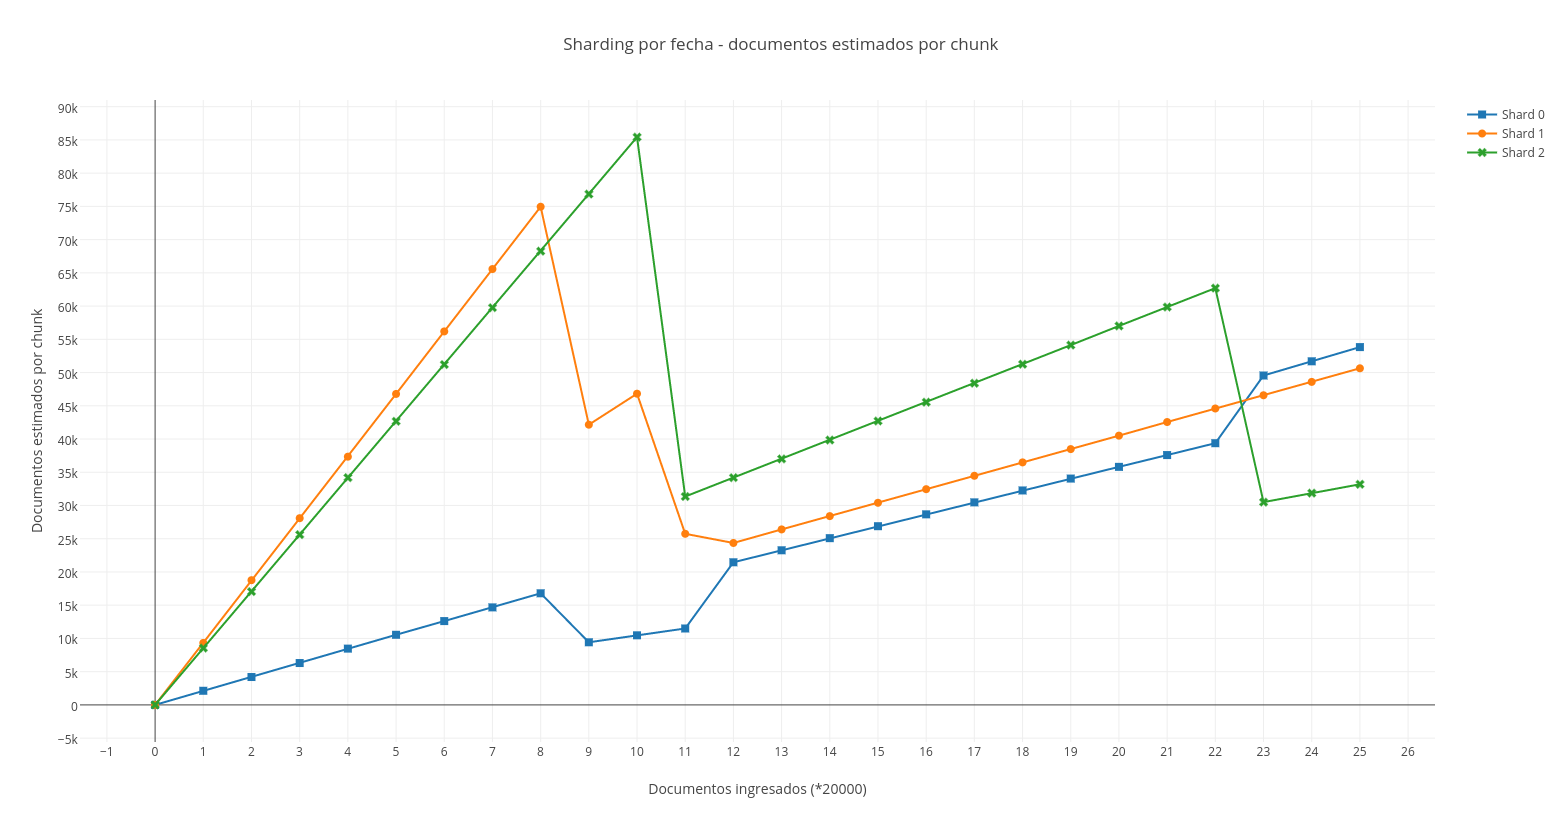
\includegraphics[scale=0.3,keepaspectratio=true]{./fecha-documentos-estimados-por-chunk.png}
 \caption{Datos por chunk}
\end{figure}

En la figura se observa la evolución del promedio de datos por chunk para cada shard, las primeras iteraciones presentan muchas fluctuaciones, debido a las divisiones y migraciones
de chunks, luego se observa como se estabiliza y se mantiene esa tendencia.

\begin{figure}[h!]
 \centering
 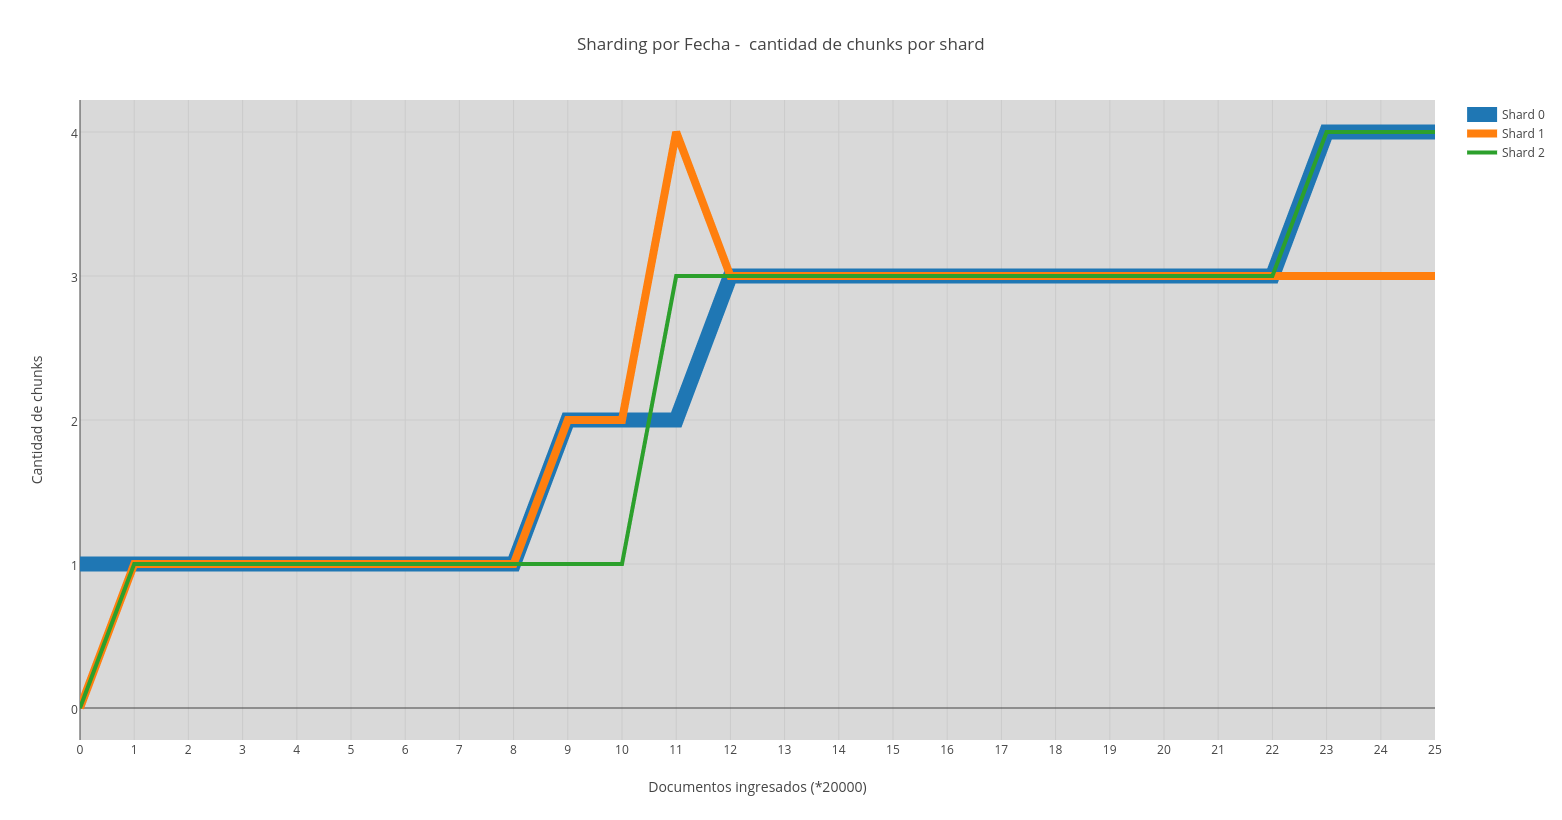
\includegraphics[scale=0.3,keepaspectratio=true]{./Fecha-cantidad-de-chunks-por-shard.png}
 \caption{Chunks por shard}
\end{figure}

Por último se muestra la cantidad de chunks por shard, permitiendo comparar mejor los gráficos anteriores.\\

Para observar mejor los gráficos se pueden acceder mediante los siguientes links a su representación online:
\begin{itemize}
 \item \href{https://plot.ly/~fzanollo/22/sharding-por-fecha-documentos-por-shard/}{Documentos por shard}
 \item \href{https://plot.ly/~fzanollo/31/sharding-por-fecha-documentos-estimados-por-chunk/}{Documentos estimados por chunk}
 \item \href{https://plot.ly/~fzanollo/47/sharding-por-fecha-cantidad-de-chunks-por-shard/}{Cantidad de chunks por shard}
\end{itemize}